%% ============================================================
%% AUV Software Documentation -- regenerated against current code
%% Compile: pdflatex AUV_Software_Documentation_v2.tex  (x2)
%% ============================================================
\documentclass[10.5pt,a4paper]{article}

\usepackage[T1]{fontenc}
\usepackage[utf8]{inputenc}
\usepackage{libertinus}
\usepackage{montserrat}
\usepackage{microtype}
\usepackage[margin=1.9cm,top=1.7cm,bottom=1.9cm]{geometry}
\usepackage{graphicx}
\usepackage{xcolor}
\usepackage{amsmath,amssymb}
\usepackage{booktabs}
\usepackage{array}
\usepackage{tabularx}
\usepackage{calc}
\usepackage{colortbl}
\usepackage{enumitem}
\usepackage{listings}
\usepackage{caption}
\captionsetup{labelformat=empty, font=small, skip=4pt}
\usepackage{tikz}
\usetikzlibrary{arrows.meta,positioning,calc,fit}
\usepackage{hyperref}
\usepackage{fancyhdr}
\usepackage{titlesec}
\usepackage{float}
\usepackage[most]{tcolorbox}
\usepackage{setspace}

\definecolor{ink}{HTML}{16233A}
\definecolor{inksoft}{HTML}{4A5568}
\definecolor{accent}{HTML}{6A3FA0}
\definecolor{accentsoft}{HTML}{F1EAFB}
\definecolor{codeorange}{HTML}{F7B267}
\definecolor{codeorangetxt}{HTML}{7A4A00}
\definecolor{hairline}{HTML}{D8DEE6}
\definecolor{tablehead}{HTML}{F3F5F7}
\definecolor{warnbg}{HTML}{FDEDEC}
\definecolor{warnbd}{HTML}{C0392B}

\hypersetup{colorlinks=true, linkcolor=accent, urlcolor=accent,
  pdftitle={AUV Software Documentation}, pdfauthor={AUV Team}}

\titleformat{\section}
  {\normalfont\fontfamily{Montserrat-TLF}\selectfont\large\bfseries\color{ink}}
  {\thesection}{0.55em}{}
  [\vspace{1pt}\textcolor{accent}{\rule{\linewidth}{1pt}}\vspace{1pt}]
\titlespacing*{\section}{0pt}{0.9em}{0.45em}
\titleformat{\subsection}
  {\normalfont\fontfamily{Montserrat-TLF}\selectfont\normalsize\bfseries\color{ink}}
  {\thesubsection}{0.55em}{}
\titlespacing*{\subsection}{0pt}{0.7em}{0.3em}
\titleformat{\subsubsection}
  {\normalfont\fontfamily{Montserrat-TLF}\selectfont\small\bfseries\color{inksoft}}
  {}{0em}{}
\titlespacing*{\subsubsection}{0pt}{0.5em}{0.2em}

\pagestyle{fancy}\fancyhf{}
\renewcommand{\headrulewidth}{0pt}
\renewcommand{\footrulewidth}{0.5pt}
\fancyfoot[L]{\footnotesize\color{inksoft}AUV Software Documentation}
\fancyfoot[R]{\footnotesize\color{inksoft}\thepage}

\newcolumntype{C}[1]{>{\centering\arraybackslash}p{#1}}
\newcolumntype{L}[1]{>{\raggedright\arraybackslash}p{#1}}
\renewcommand{\arraystretch}{1.25}
\setlength{\parskip}{3.4pt}
\setlength{\parindent}{0pt}

% inline "highlighted code" span, like the reference document's tan/orange chips
\newcommand{\hl}[1]{\tikz[baseline=(t.base)]{\node[fill=codeorange,rounded corners=2pt,inner sep=2pt,font=\ttfamily\scriptsize,text=codeorangetxt] (t) {#1};}}
\newcommand{\code}[1]{\texttt{\small\color{accent}#1}}

\tcbuselibrary{skins,breakable}
\newtcolorbox{notebox}[1][]{colback=accentsoft, colframe=accent, coltitle=white,
  boxrule=0.7pt, fonttitle=\fontfamily{Montserrat-TLF}\bfseries\small, title={Note}, rounded corners,
  left=6pt,right=6pt,top=3pt,bottom=3pt, #1}

% ---- FSM / topology diagram box styles (purple, matching reference figures) --
\tikzset{
  fsmbox/.style={rectangle,rounded corners=3pt,draw=accent,line width=1pt,
    fill=accentsoft,text=ink,align=center,font=\scriptsize,
    minimum height=0.62cm,text width=3.55cm,inner sep=3pt},
  topobox/.style={rectangle,rounded corners=3pt,draw=accent,line width=0.9pt,
    fill=accentsoft,text=ink,align=center,font=\scriptsize,
    minimum height=0.55cm,text width=2.35cm,inner sep=2.5pt},
  fsmarr/.style={-Stealth,line width=0.9pt,color=ink},
  fsmlabel/.style={font=\tiny\itshape,color=inksoft},
}

\begin{document}

%% ============================================================
\section{Description of Software Architecture}

The AUV's software stack runs on \textbf{ROS\,2 Jazzy}. The workspace is split into ten
packages under \hl{auv\_ws/src/} -- \hl{auv\_vision}, \hl{auv\_planner}, \hl{auv\_telemetry},
\hl{auv\_description}, \hl{auv\_bringup}, plus four packages currently scaffolded but not
yet implemented (\hl{auv\_controls}, \hl{auv\_propulsion}, \hl{auv\_sensors}, \hl{auv\_msgs} --
each holds only a \code{CMakeLists.txt}/\code{package.xml}, no source) and \hl{auv\_teleop}
(also an empty stub). Every inter-node link is an asynchronous ROS\,2 topic.

\begin{figure}[H]
\centering
\begin{lstlisting}[basicstyle=\ttfamily\scriptsize,frame=single,framesep=5pt,
  rulecolor=\color{hairline},backgroundcolor=\color{tablehead},breaklines=true]
auv_ws/src/
|-- auv_bringup/           launch/ (sim_mission.launch.py, sim_post_gate.launch.py)
|                           config/ (sim_params.yaml, real_params.yaml)
|-- auv_description/       urdf/, meshes/, models/auv_box/model.sdf, launch/bridge.launch.py
|-- auv_vision/
|   |-- gate_detector_node.py          |-- blue_bin_cv_detector_node.py
|   |-- gate_localizer_node.py         |-- blue_bin_localizer_node.py
|   |-- blue_bin_detector_node.py      |-- green_detector_node.py
|   |-- green_localizer_node.py        |-- underwater_view_node.py
|   `-- bottom_cam_altitude_test.py    (test-harness script, not a mission node)
|-- auv_planner/
|   |-- gate_navigator_v2_node.py      (launched -- one-pass gate crossing)
|   |-- gate_navigator_node.py         (legacy round-trip FSM, kept but unused)
|   `-- green_navigator_node.py
|-- auv_telemetry/
|   |-- mission_logger_node.py  |-- mission_monitor_node.py  |-- trail_mapper_node.py
|-- auv_controls/          [EMPTY STUB -- reserved for closed-loop cmd_vel PID]
|-- auv_propulsion/        [EMPTY STUB -- reserved for thruster allocation]
|-- auv_sensors/           [EMPTY STUB -- reserved for EKF / real-hardware drivers]
|-- auv_msgs/               [EMPTY STUB -- no custom interfaces defined; std msgs only]
`-- auv_teleop/             [EMPTY STUB]
\end{lstlisting}
\caption{Fig 1. Workspace layout as built (10 packages; four are empty stub packages reserved for Phase 2).}
\end{figure}

Unlike the planned overactuated 8-thruster vehicle, the vehicle currently in the
simulation is driven \emph{kinematically}: Gazebo's \code{gz-sim-velocity-control-system}
plugin sets body velocity directly from \code{/model/auv\_box/cmd\_vel}, so
\hl{auv\_controls} and \hl{auv\_propulsion} have nothing to run yet -- this is a deliberate,
documented placeholder (see Section~6), not an omission.

%% ============================================================
\section{Salient Features of the Software Stack}

\begin{itemize}[leftmargin=1.3em,itemsep=2pt]
  \item \textbf{Kinematic Velocity-Controlled Simulation (\hl{auv\_description}):} The AUV
    tracks \code{cmd\_vel} exactly via Gazebo's built-in \code{VelocityControl} plugin. A
    Fossen-model hydrodynamics plugin (BlueROV2 drag coefficients) is already attached to
    the hull but currently has \emph{no effect} on motion -- it activates automatically the
    moment the velocity-control plugin is swapped for individual thrusters in Phase 2.
  \item \textbf{Stereo-Vision Based 3D Localization (\hl{auv\_vision}):} Gate and green-mat
    3D coordinates are computed by correlating YOLOv8n boxes (gate) / HSV contours (mat)
    with \code{stereo\_image\_proc} disparity maps. The gate localizer interrogates four
    prioritized candidate points across a 9$\times$9 disparity patch (Left Pole $\to$ Right
    Pole $\to$ Crossbar $\to$ Center), takes the median of valid pixels, and applies
    $depth = f_x \cdot B / disparity$ with a plausibility guard (0.2\,m--19.1\,m).
  \item \textbf{Dual-Camera Cross-Handoff:} The front stereo pair handles long-range
    acquisition of the gate and green mat; the downward camera takes over for the blue-bin
    approach and fine centering, using odometry altitude for pinhole projection instead of
    stereo disparity.
  \item \textbf{Dead-Reckoning Visual Fallback (\hl{auv\_planner}):} Both navigators freeze
    the last verified target position in the odom frame and continue driving toward it when
    the live YOLO/HSV feed goes stale, then reconcile with fresh detections as they arrive.
  \item \textbf{HSV-Based False-Positive Reduction:} \hl{blue\_bin\_cv\_detector\_node}
    (bottom camera) only accepts a blue blob if $\geq$15\% of its pixel area overlaps a
    dilated green-mat mask in the same frame -- open blue pool water cannot pass this check,
    eliminating false positives with zero additional training data.
  \item \textbf{Advance-and-Sweep Search:} Rather than a fixed search radius, both the gate
    (lateral only) and green/blue-bin (lateral \emph{plus} forward creep) searches strafe
    $\pm$ a bound, reverse at each limit, and -- for the post-gate searches -- creep forward
    and repeat if a full pass finds nothing, up to a bounded total-advance budget.
  \item \textbf{Post-Mission Trail Mapping \& Live Dashboard (\hl{auv\_telemetry}):}
    \hl{trail\_mapper\_node} records a pose whenever the AUV has moved $\geq$0.10\,m,
    re-exports a colour-coded top-down PNG and an interactive 3D Plotly HTML map every 30\,s
    and on shutdown, while \hl{mission\_monitor\_node} renders a live ANSI terminal
    dashboard.
  \item \textbf{No active safety envelope yet:} tilt damping, a depth envelope, and wall
    repulsion are not implemented in the current controller -- there \emph{is} no standalone
    controller node; they are natural additions once \hl{auv\_controls} is built out.
\end{itemize}

%% ============================================================
\section{Logical Steps in the Working of Software Components}

Mission planning lives in \hl{auv\_planner}: \hl{gate\_navigator\_v2\_node} (the FSM actually
launched by \code{sim\_mission.launch.py}) for gate traversal, and
\hl{green\_navigator\_node} for everything after the gate.

\subsection{Gate Navigation (\texttt{gate\_navigator\_v2\_node})}

\begin{figure}[H]\centering
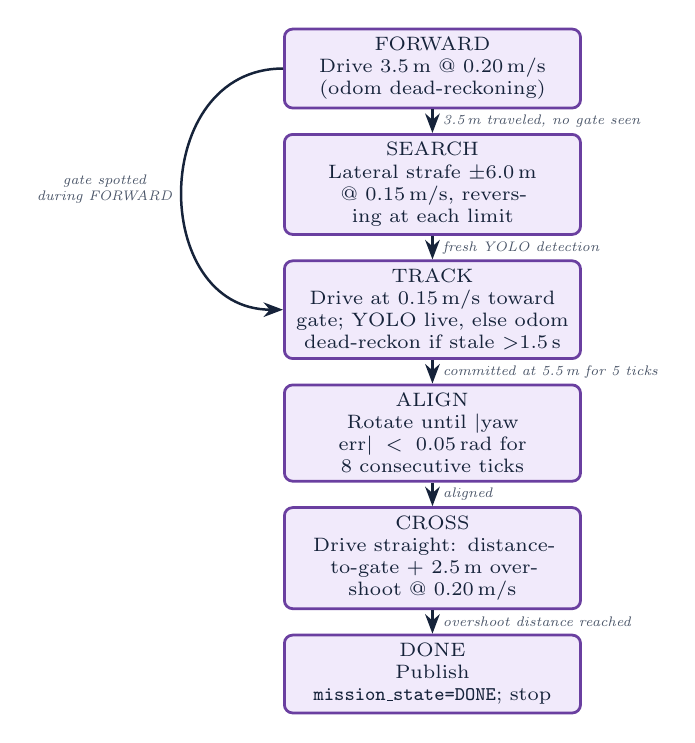
\begin{tikzpicture}[node distance=0.30cm and 1.6cm]
  \node[fsmbox] (fwd)  {FORWARD\\Drive 3.5\,m @ 0.20\,m/s (odom dead-reckoning)};
  \node[fsmbox, below=of fwd] (srch) {SEARCH\\Lateral strafe $\pm$6.0\,m @ 0.15\,m/s, reversing at each limit};
  \node[fsmbox, below=of srch] (trk) {TRACK\\Drive at 0.15\,m/s toward gate; YOLO live, else odom dead-reckon if stale $>$1.5\,s};
  \node[fsmbox, below=of trk] (aln) {ALIGN\\Rotate until $\vert$yaw err$\vert<0.05$\,rad for 8 consecutive ticks};
  \node[fsmbox, below=of aln] (crs) {CROSS\\Drive straight: distance-to-gate + 2.5\,m overshoot @ 0.20\,m/s};
  \node[fsmbox, below=of crs] (done) {DONE\\Publish \texttt{mission\_state=DONE}; stop};
  \draw[fsmarr] (fwd) -- (srch) node[midway,right,fsmlabel]{3.5\,m traveled, no gate seen};
  \draw[fsmarr] (srch) -- (trk) node[midway,right,fsmlabel]{fresh YOLO detection};
  \draw[fsmarr] (trk) -- (aln) node[midway,right,fsmlabel]{committed at 5.5\,m for 5 ticks};
  \draw[fsmarr] (aln) -- (crs) node[midway,right,fsmlabel]{aligned};
  \draw[fsmarr] (crs) -- (done) node[midway,right,fsmlabel]{overshoot distance reached};
  \draw[fsmarr] (fwd.west) .. controls +(-1.7,0) and +(-1.7,0) .. (trk.west)
    node[midway,left,fsmlabel,align=center]{gate spotted\\during FORWARD};
\end{tikzpicture}
\caption{Fig 2. Gate Navigator State Machine (\texttt{auv\_planner/gate\_navigator\_v2\_node}) -- values as configured in \texttt{sim\_params.yaml}.}
\end{figure}

The legacy \hl{gate\_navigator\_node} (round-trip crossing with a U-turn and return leg) is
still present in the package but is \emph{not} referenced by \code{sim\_mission.launch.py};
switching to it is a one-line \code{executable=} change.

\subsection{Post-Gate Navigation (\texttt{green\_navigator\_node})}

Once \hl{gate\_navigator\_v2\_node} publishes \code{DONE}, \hl{green\_navigator\_node} runs
an 11-state FSM -- longer than a simple search/approach/centre pipeline because the mat and
bin can sit well beyond camera range and the AUV must actively creep to find them:

\begin{figure}[H]\centering
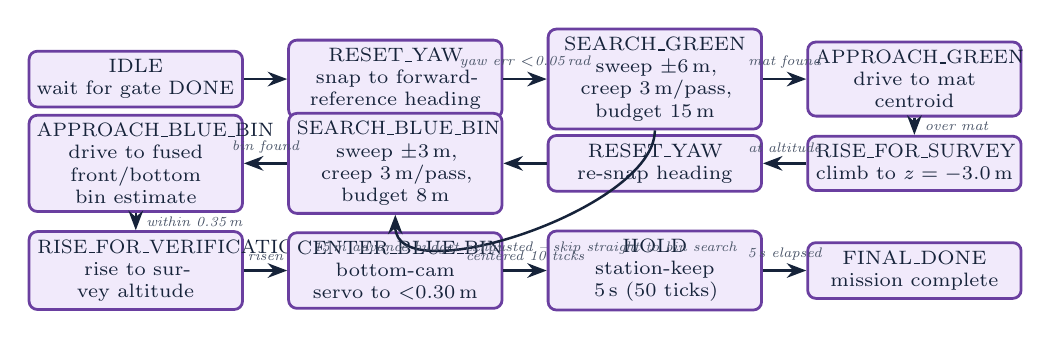
\begin{tikzpicture}[node distance=0.22cm and 0.55cm]
  \node[fsmbox,text width=2.5cm] (idle) {IDLE\\wait for gate DONE};
  \node[fsmbox,text width=2.5cm,right=of idle] (ry1) {RESET\_YAW\\snap to forward-reference heading};
  \node[fsmbox,text width=2.5cm,right=of ry1] (sg) {SEARCH\_GREEN\\sweep $\pm$6\,m, creep 3\,m/pass, budget 15\,m};
  \node[fsmbox,text width=2.5cm,right=of sg] (ag) {APPROACH\_GREEN\\drive to mat centroid};
  \node[fsmbox,text width=2.5cm, below=of ag] (rfs) {RISE\_FOR\_SURVEY\\climb to $z=-3.0$\,m};
  \node[fsmbox,text width=2.5cm, left=of rfs] (ry2) {RESET\_YAW\\re-snap heading};
  \node[fsmbox,text width=2.5cm, left=of ry2] (sb) {SEARCH\_BLUE\_BIN\\sweep $\pm$3\,m, creep 3\,m/pass, budget 8\,m};
  \node[fsmbox,text width=2.5cm, left=of sb] (ab) {APPROACH\_BLUE\_BIN\\drive to fused front/bottom bin estimate};
  \node[fsmbox,text width=2.5cm, below=of ab] (rfv) {RISE\_FOR\_VERIFICATION\\rise to survey altitude};
  \node[fsmbox,text width=2.5cm, right=of rfv] (cb) {CENTER\_BLUE\_BIN\\bottom-cam servo to $<$0.30\,m};
  \node[fsmbox,text width=2.5cm, right=of cb] (hold) {HOLD\\station-keep 5\,s (50 ticks)};
  \node[fsmbox,text width=2.5cm, right=of hold] (fd) {FINAL\_DONE\\mission complete};

  \draw[fsmarr] (idle) -- (ry1);
  \draw[fsmarr] (ry1) -- (sg) node[midway,above,fsmlabel]{yaw err $<$0.05\,rad};
  \draw[fsmarr] (sg) -- (ag) node[midway,above,fsmlabel]{mat found};
  \draw[fsmarr] (ag) -- (rfs) node[midway,right,fsmlabel]{over mat};
  \draw[fsmarr] (rfs) -- (ry2) node[midway,above,fsmlabel]{at altitude};
  \draw[fsmarr] (ry2) -- (sb);
  \draw[fsmarr] (sb) -- (ab) node[midway,above,fsmlabel]{bin found};
  \draw[fsmarr] (ab) -- (rfv) node[midway,right,fsmlabel]{within 0.35\,m};
  \draw[fsmarr] (rfv) -- (cb) node[midway,above,fsmlabel]{risen};
  \draw[fsmarr] (cb) -- (hold) node[midway,above,fsmlabel]{centered 10 ticks};
  \draw[fsmarr] (hold) -- (fd) node[midway,above,fsmlabel]{5\,s elapsed};
  \draw[fsmarr] (sg.south) .. controls +(0,-1.0) and +(0,-1.0) .. (sb.south)
    node[midway,below,fsmlabel]{15\,m advance budget exhausted -- skip straight to bin search};
\end{tikzpicture}
\caption{Fig 3. Post-Gate Navigator State Machine (\texttt{auv\_planner/green\_navigator\_node}) -- 11 states, values as configured in \texttt{sim\_params.yaml}. There is no separate \texttt{CLEAR\_GATE} surge state; \texttt{RESET\_YAW} runs immediately on the gate's \texttt{DONE}.}
\end{figure}

\begin{notebox}
Two robustness details not visible in the diagram: the blue-bin odom estimate is fused from
whichever camera is more reliable at the time (front-camera one-shot depth $+1.0$\,m fudge
until the bottom camera gets a confirmed-over-green reading), and \texttt{CENTER\_BLUE\_BIN}
uses a leaky tick counter (drains by 1 on a bad tick instead of resetting to 0) so a single
missed frame cannot restart the centering streak.
\end{notebox}

%% ============================================================
\section{Dataset Preparation and Object Classes}

\subsection{Data Sources}

\textbf{Simulation-Generated Images:} The competition arena is built in Gazebo Harmonic
(PVC gate, 8\,m$\times$2\,m green target mat, blue drum). \hl{bottom\_cam\_altitude\_test.py}
is a standalone test-harness script (not a launched mission node) that teleports the AUV
across a fixed grid of 5 altitudes ($z\in\{-2.0,-2.5,-3.0,-3.5,-4.0\}$\,m) $\times$ 6 named
horizontal offsets (over-bin, $\pm$1\,m left/right, +2\,m right, 1\,m forward, 1.5\,m back)
-- 30 teleport poses per capture pass -- saving annotated bottom-camera frames to
\code{\textasciitilde/auv\_ws/bottom\_cam\_test/}.

\textbf{Kaggle and External Sources:} Underwater imagery from Kaggle supplements the
simulation captures with real turbidity, backscatter, and lighting variation.

\subsection{Object Classes in the Dataset}

The trained YOLOv8n weights (\texttt{gate\_detection\_v8.pt}, loaded by
\hl{gate\_detector\_node}) are multi-class -- confirmed by the class-ID map used in the
detector nodes and matching the confusion matrix in Fig.~4 -- but \textbf{only two of those
classes are currently wired into the ROS graph}: the red-bin and QR-code classes have no
corresponding detector/localizer nodes yet.

\begin{table}[H]\centering\small
\begin{tabularx}{\textwidth}{L{2.1cm} X L{5.0cm}}
\toprule
\rowcolor{tablehead}\textbf{Class} & \textbf{Geometry} & \textbf{Current ROS integration} \\
\midrule
Gate & Two vertical PVC posts + crossbar; camera\_test.sdf posts at 3.0\,m spacing & \textbf{Live:} YOLOv8n (class 3) + 4-candidate stereo disparity \\
Blue Bin & Cylindrical drum, 0.3\,m radius, 0.5\,m height, on the green mat & \textbf{Live:} YOLOv8n (class 1, front) + HSV green-overlap (bottom) \\
Red Bin & Same geometry as blue bin & Trained in the model (class 0) but \textbf{no red\_bin\_detector / red\_bin\_localizer node exists} in \texttt{auv\_vision} \\
QR Code & Floor-mounted payload marker & Trained in the model (class 2) but \textbf{no qr\_detector / qr\_localizer node exists} \\
Green Target Mat & 8\,m $\times$ 2\,m floor mat & Classical HSV segmentation (no YOLO class -- by design) \\
\bottomrule
\end{tabularx}
\caption{Table: object classes trained vs. classes actually consumed by a running node today.}
\end{table}

\subsection{Model Details}

YOLOv8n (nano) is the shared detection backbone for both the gate and blue-bin detectors.
The green mat uses classical HSV thresholding with morphological cleanup exclusively --
no neural inference is run for it. Fig.~4 and Fig.~5 below are the training artifacts for
the currently-loaded weights and are unchanged from the underlying training run.

Six checkpoints are retained side-by-side in \hl{auv\_vision/weights/}
(\code{gate\_detection\_v2/v4/v5/v6/v7/v8.pt}), spanning class-ID remaps as the label set grew
-- \hl{gate\_detector\_node} loads \code{v8.pt} (gate = class 3) while
\hl{blue\_bin\_detector\_node} loads the earlier \code{v7.pt} (blue bin = class 1); the two
detector nodes are pinned to different checkpoints rather than sharing one, so a future
retrain has to keep both class maps in mind or update both \code{model\_weights} parameters
together.

\begin{notebox}[title={Live Detection Capture (a byproduct, not a re-training pipeline)}]
Every detector node also writes debug frames during normal operation, which incidentally
accumulates more real candidate training data as missions are run:
\hl{gate\_detector\_node} overwrites a single \code{latest\_detection.jpg} in
\code{\textasciitilde/.ros/yolo\_debug/}; \hl{blue\_bin\_detector\_node} keeps every
individual detection, numbered and confidence-tagged, in a fresh
\code{\textasciitilde/.ros/blue\_bin\_detections/run\_\textless timestamp\textgreater/} folder
per launch; \hl{blue\_bin\_cv\_detector\_node} and \hl{green\_detector\_node} each overwrite one
annotated frame showing their HSV mask overlay. None of this feeds an automated re-training
loop today -- it exists purely for live debugging.
\end{notebox}

\begin{figure}[H]\centering
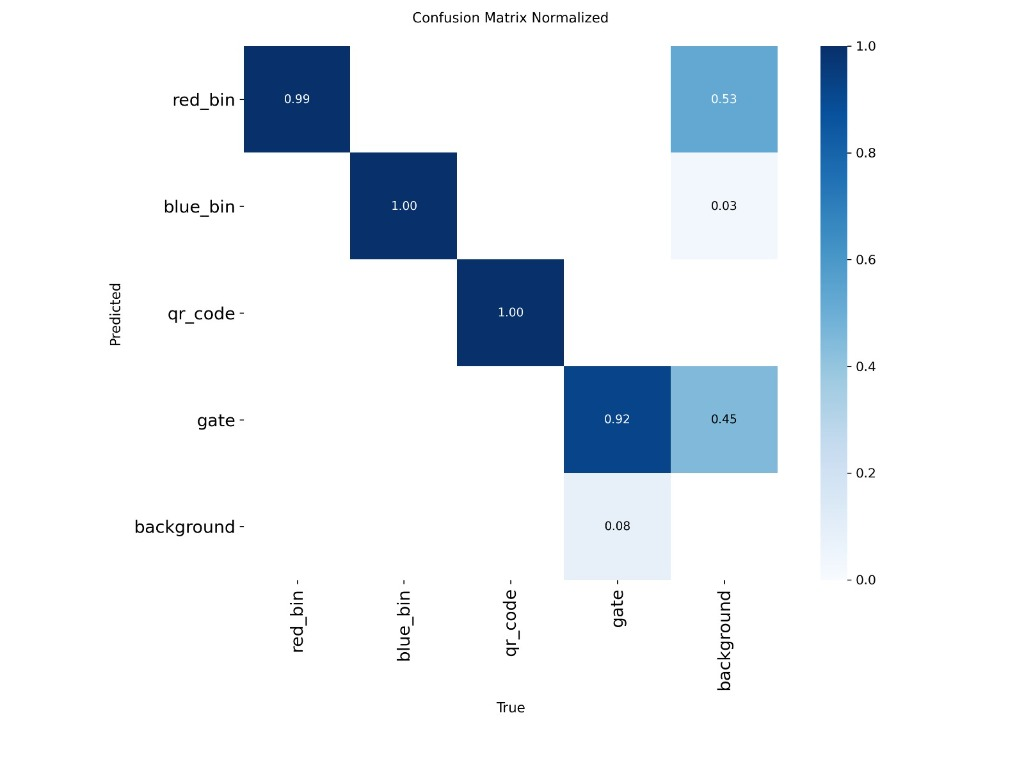
\includegraphics[width=0.46\textwidth]{photos_v2/fig4_confusion_matrix.jpg}\\[2pt]
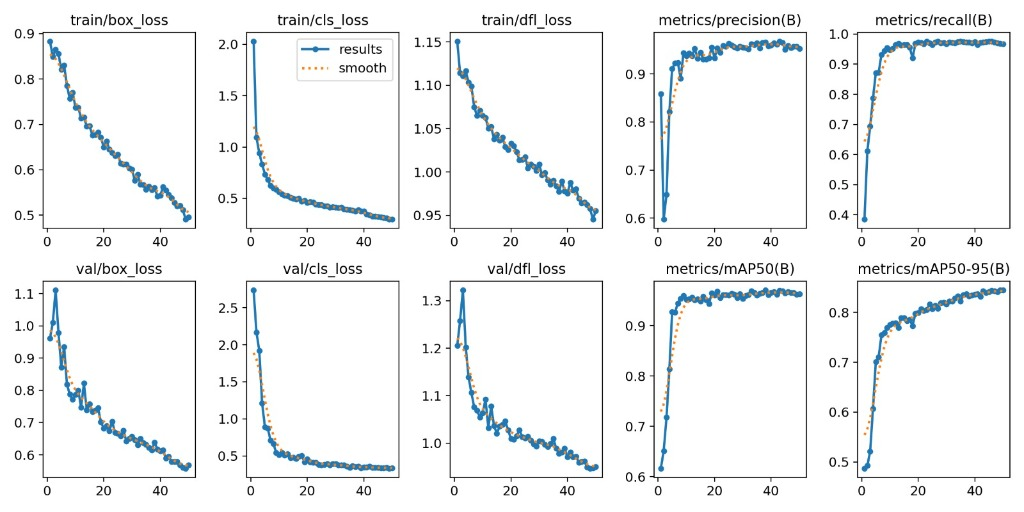
\includegraphics[width=0.82\textwidth]{photos_v2/fig5_training_metrics.jpg}
\caption{Fig 4/5. YOLOv8n training confusion matrix and loss/precision/recall/mAP curves for the weights currently loaded by \texttt{gate\_detector\_node} and \texttt{blue\_bin\_detector\_node}.}
\end{figure}

%% ============================================================
\section{Object Detection and Vision Pipeline}

\subsection{Gate Detection Pipeline}

\hl{gate\_detector\_node} subscribes to \code{/model/auv\_box/stereo\_front/left/image\_raw},
runs YOLOv8n at confidence 0.10, and publishes the single highest-confidence box to
\code{/auv/gate\_detection\_2d}. \hl{gate\_localizer\_node} fuses this with
\code{stereo\_image\_proc} disparity: it samples a 9$\times$9 patch at each of Left Pole,
Right Pole, Crossbar, Center (in that priority order), accepts the first with $\geq$3 valid
pixels, and computes $Z = f_xB/d$, $X=(u-c_x)Z/f_x$, $Y=(v-c_y)Z/f_y$ (baseline
$B=0.075$\,m as configured in \code{sim\_params.yaml}), guarded to 0.2--19.1\,m, publishing
\code{[x,y,z,conf]} to \code{/auv/gate\_position\_3d}.

\subsection{Blue Bin Detection Pipeline}

\hl{blue\_bin\_detector\_node} runs YOLOv8n (class 1) on \emph{both} the front and bottom
camera feeds (conf $\geq$0.70), publishing to
\code{/auv/blue\_bin\_detection\_\{front,bottom\}\_2d}. \hl{blue\_bin\_cv\_detector\_node}
replaces the bottom-camera YOLO path with an HSV blue/green overlap test ($\geq$15\%
overlap with a dilated green mask) on the same topic, so open water cannot false-positive.
\hl{blue\_bin\_localizer\_node} prefers the bottom-camera altitude projection when a
confident bottom detection exists, else falls back to a front-camera stereo slant-range
estimate.

\subsection{Green Mat Detection Pipeline}

\hl{green\_detector\_node} applies HSV segmentation ($H{:}38\text{--}82$, $S{:}80\text{--}255$,
$V{:}60\text{--}255$). On the front camera it only processes the bottom 40\% of the frame
(\code{front\_roi\_top\_frac=0.60}), since the mat only ever appears low in that
horizontally-mounted camera's field of view; the bottom camera processes the full frame and
reports a coverage fraction used as the Phase-1/Phase-2 handoff signal in
\hl{green\_localizer\_node}.

\subsection{Underwater View Rendering}

\hl{underwater\_view\_node} applies Beer--Lambert attenuation
($I_\lambda = e^{-\alpha_\lambda r}I_{0,\lambda} + (1-e^{-\alpha_\lambda r})\,\text{bg}_\lambda$)
to the left camera feed using the disparity-derived range, publishing a separate,
display-only \code{/auv/underwater\_view/image\_raw} topic -- every detector still reads the
raw, un-hazed feed. This exists because Gazebo Harmonic's \code{<fog>} tag is a no-op and the
world's water volume cannot tint a camera sitting inside it.

\begin{notebox}
\textbf{Not yet implemented:} \code{red\_bin\_detector\_node}, \code{red\_bin\_localizer\_node},
\code{qr\_detector\_node}, \code{qr\_localizer\_node}. The trained model already supports the
classes; only the ROS wiring is missing.
\end{notebox}

%% ============================================================
\section{Controls, Propulsion \& Thruster Allocation}

\textbf{This section differs the most from the vehicle's eventual design.} There is
currently no closed-loop velocity controller node and no thruster-allocation node in the
software stack -- \hl{auv\_controls} and \hl{auv\_propulsion} are empty package stubs
(\code{CMakeLists.txt} + \code{package.xml} only). Motion is produced directly by Gazebo:

\begin{itemize}[leftmargin=1.3em,itemsep=2pt]
  \item \textbf{\code{gz-sim-velocity-control-system}} reads
    \code{/model/auv\_box/cmd\_vel} (a \code{geometry\_msgs/Twist} published by whichever
    navigator is active) and sets the model's body velocity \emph{directly}, every physics
    step -- perfect velocity tracking, no PID, no thruster forces.
  \item \textbf{\code{gz-sim-hydrodynamics-system}} is attached to \code{base\_link} with
    Fossen-model added-mass and quadratic-drag coefficients taken from the published BlueROV2
    values ($X_{u|u|}{=}{-}33.7$, $Y_{v|v|}{=}{-}54.2$, $Z_{w|w|}{=}{-}73.2$, roll/pitch/yaw
    drag ${=}{-}4.0$). These coefficients currently have \textbf{zero effect} on motion,
    because \code{VelocityControl} overwrites the resulting forces every step -- they exist
    pre-wired so that removing the velocity-control plugin is the only change needed to make
    drag real.
  \item The eight thruster meshes (\code{Thruster\_1.STL}~--~\code{Thruster\_8.STL}) are
    present visually on the model but have \textbf{no joints or links} in \code{model.sdf} --
    they render but do not actuate.
\end{itemize}

\begin{notebox}[title={Documented Phase-2 Path (from \texttt{model.sdf} comments)}]
(1) Remove the \code{VelocityControl} plugin. (2) Add one
\code{gz-sim-thruster-system} per thruster, joined to the existing meshes. (3) Implement
Moore-Penrose thrust allocation in \hl{auv\_propulsion}. (4) Implement a closed-loop
\code{cmd\_vel} PID in \hl{auv\_controls} so the navigators' existing \code{Twist} interface
needs no changes. Only after step 1 do the hydrodynamics coefficients above start affecting
the vehicle.
\end{notebox}

No tilt-damping, depth-envelope, or wall-repulsion safety logic exists anywhere in the
current stack; these are natural additions to the not-yet-built \hl{auv\_controls} node.

%% ============================================================
\section{Sensor Suite, State Estimation \& Sim-to-Real Portability}

\subsection{Sensor Suite \& Camera Specifications}

\begin{table}[H]\centering\small
\begin{tabularx}{\textwidth}{L{2.6cm} L{4.0cm} L{3.1cm} X}
\toprule
\rowcolor{tablehead}\textbf{Sensor} & \textbf{Topic} & \textbf{Rate / Res.} & \textbf{Role} \\
\midrule
Stereo Front Pair & \scriptsize\ttfamily .../stereo\_front/\{L,R\}/image\_raw & 15\,Hz\newline 640$\times$480, HFOV 73$^\circ$ & Gate \& green-mat long-range 3D localization \\
Downward Camera & \scriptsize\ttfamily .../bottom/image\_raw & 15\,Hz\newline 640$\times$480, HFOV 73$^\circ$ & Blue-bin/green-mat close-range tracking and centering \\
Ground-truth Odometry & \scriptsize\ttfamily /auv/odom & 50\,Hz & Position, orientation, twist -- consumed by every navigator, localizer, and logger \\
\bottomrule
\end{tabularx}
\end{table}

There is \textbf{no IMU and no separate depth sensor} modeled in \code{model.sdf} today --
depth comes from the Z channel of the ground-truth odometry published by
\code{gz-sim-odometry-publisher-system} (\code{odom\_frame=map}, \code{robot\_base\_frame=}
\code{base\_link}, 50\,Hz).

\subsection{State Estimation}

\hl{auv\_sensors} is an empty stub package: there is currently \textbf{no Extended Kalman
Filter and no \code{robot\_localization} node running}. The stack relies entirely on
Gazebo's ground-truth odometry. \code{real\_params.yaml} already anticipates the switch --
it sets \code{trail\_mapper\_node.odom\_frame: 'odom'} with a comment noting that real
hardware will source it from a \code{robot\_localization} EKF -- but no launch file or EKF
config exists yet to consume it.

\subsection{Sim-to-Real Configuration Isolation}

Tunable node parameters are isolated in \hl{auv\_bringup/config/}: \code{sim\_params.yaml}
(loaded by \code{sim\_mission.launch.py}) and \code{real\_params.yaml} (parameter values
only, pre-written for hardware but not yet wired to a hardware launch file -- there is no
\code{mission.launch.py} in the workspace yet). Node source code is unchanged between the
two; only YAML values differ (e.g. \code{cross\_speed} drops from 0.20 to 0.15\,m/s, and
\code{track\_speed}/\code{search\_spin\_speed} are lowered for a conservative first real run).

%% ============================================================
\section{Software Used}

\begin{table}[H]\centering\small
\begin{tabularx}{\textwidth}{L{4cm} X}
\toprule
\rowcolor{tablehead}\textbf{Component} & \textbf{Purpose in this stack} \\
\midrule
ROS\,2 Jazzy & Core middleware -- node lifecycle, DDS pub/sub, launch, parameters. \\
Ultralytics YOLOv8n & Gate and blue-bin bounding-box detection. \\
OpenCV (\code{cv\_bridge}) & Image conversion, HSV thresholding/contours, Beer-Lambert haze rendering. \\
Gazebo Harmonic & Physics simulation; \code{VelocityControl} kinematic drive + inert Hydrodynamics plugin. \\
\code{stereo\_image\_proc} & Stereo rectification and disparity generation from the front camera pair. \\
\code{ros\_gz\_bridge} / \code{ros\_gz\_image} & Bridges Gazebo image, odometry, and \code{cmd\_vel} topics into ROS\,2. \\
Matplotlib / Plotly & Post-mission 2D PNG and interactive 3D HTML trajectory maps. \\
Python 3 & Every custom node is pure Python. \\
\bottomrule
\end{tabularx}
\end{table}
{\sloppy\small\itshape Not currently in the runtime stack, despite being anticipated in
comments/config: \code{robot\_localization} (EKF) and \code{gz-sim-thruster-system}
(per-thruster physics).\par}

%% ============================================================
\section{Sensor and Communication Circuit (Software Topology)}

Raw optical streams from the front stereo pair and bottom camera split into YOLO/HSV
detection paths and the disparity depth path, merging at the localizer nodes to produce 3D
coordinates. The two diagrams below are drawn directly from the subscriptions/publications
declared in each node's source -- not from the aspirational pipeline in earlier drafts of
this document.

\begin{figure}[H]\centering
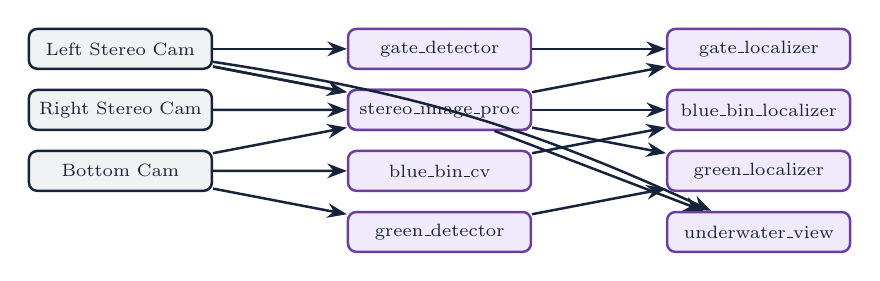
\begin{tikzpicture}[scale=0.92, every node/.append style={scale=0.92}, node distance=0.24cm and 0.5cm]
  \node[topobox,fill=ink!6,draw=ink] (lc) {Left Stereo Cam};
  \node[topobox,fill=ink!6,draw=ink, below=of lc] (rc) {Right Stereo Cam};
  \node[topobox,fill=ink!6,draw=ink, below=of rc] (bc) {Bottom Cam};

  \node[topobox, right=1.7cm of lc] (gd) {gate\_detector};
  \node[topobox, below=of gd] (bbd) {blue\_bin\_detector};
  \node[topobox, below=of bbd] (bbcv) {blue\_bin\_cv};
  \node[topobox, below=of bbcv] (grd) {green\_detector};
  \node[topobox, right=1.7cm of rc] (sp) {stereo\_image\_proc};

  \node[topobox, right=1.7cm of gd] (gl) {gate\_localizer};
  \node[topobox, below=of gl] (bl) {blue\_bin\_localizer};
  \node[topobox, below=of bl] (grl) {green\_localizer};
  \node[topobox, below=of grl] (uw) {underwater\_view};

  \draw[fsmarr] (lc) -- (gd);
  \draw[fsmarr] (lc) -- (bbd);
  \draw[fsmarr] (lc) -- (sp);
  \draw[fsmarr] (rc) -- (sp);
  \draw[fsmarr] (bc) -- (bbd);
  \draw[fsmarr] (bc) -- (bbcv);
  \draw[fsmarr] (bc) -- (grd);
  \draw[fsmarr] (gd) -- (gl);
  \draw[fsmarr] (sp) -- (gl);
  \draw[fsmarr] (sp) -- (grl);
  \draw[fsmarr] (sp) -- (uw);
  \draw[fsmarr] (lc) to[bend left=8] (uw);
  \draw[fsmarr] (bbd) -- (bl);
  \draw[fsmarr] (bbcv) -- (bl);
  \draw[fsmarr] (grd) -- (grl);
\end{tikzpicture}
\caption{Fig 6. Perception Pipeline Topology (\texttt{auv\_vision}) -- as built: no
red-bin or QR branches exist; \texttt{blue\_bin\_localizer} fuses two independent bottom-camera
detectors (YOLO and HSV) with the front-camera YOLO path.}
\end{figure}

\begin{figure}[H]\centering
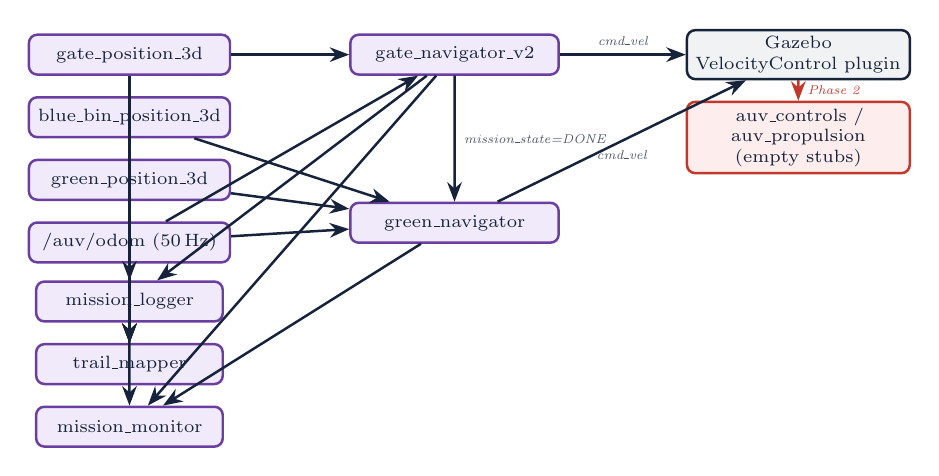
\begin{tikzpicture}[scale=0.92, every node/.append style={scale=0.92}, node distance=0.26cm and 0.65cm]
  \node[topobox,text width=2.6cm] (g3) {gate\_position\_3d};
  \node[topobox,text width=2.6cm, below=of g3] (b3) {blue\_bin\_position\_3d};
  \node[topobox,text width=2.6cm, below=of b3] (gr3) {green\_position\_3d};
  \node[topobox,text width=2.6cm, below=of gr3] (od) {/auv/odom (50\,Hz)};

  \node[topobox,text width=2.7cm, right=1.5cm of g3] (gnv) {gate\_navigator\_v2};
  \node[topobox,text width=2.7cm, below=1.6cm of gnv] (grn) {green\_navigator};

  \node[topobox,text width=2.9cm, right=1.6cm of gnv, fill=ink!6, draw=ink] (vc) {Gazebo\\VelocityControl plugin};
  \node[topobox,text width=2.9cm, below=of vc, fill=warnbg, draw=warnbd] (stub) {auv\_controls /\\auv\_propulsion\\(empty stubs)};

  \node[topobox,text width=2.4cm, below=2.6cm of g3] (log) {mission\_logger};
  \node[topobox,text width=2.4cm, below=of log] (map) {trail\_mapper};
  \node[topobox,text width=2.4cm, below=of map] (mon) {mission\_monitor};

  \draw[fsmarr] (g3) -- (gnv);
  \draw[fsmarr] (b3) -- (grn);
  \draw[fsmarr] (gr3) -- (grn);
  \draw[fsmarr] (od) -- (gnv);
  \draw[fsmarr] (od) -- (grn);
  \draw[fsmarr] (gnv) -- node[above,fsmlabel]{cmd\_vel} (vc);
  \draw[fsmarr] (grn) -- node[below,fsmlabel]{cmd\_vel} (vc);
  \draw[fsmarr] (gnv) -- node[right,fsmlabel]{mission\_state=DONE} (grn);
  \draw[fsmarr,dashed,color=warnbd] (vc) -- (stub) node[midway,right,fsmlabel,color=warnbd]{Phase 2};
  \draw[fsmarr] (gnv) -- (log);
  \draw[fsmarr] (od) -- (log);
  \draw[fsmarr] (od) -- (map);
  \draw[fsmarr] (g3) -- (map);
  \draw[fsmarr] (b3) -- (map);
  \draw[fsmarr] (gr3) -- (map);
  \draw[fsmarr] (od) -- (mon);
  \draw[fsmarr] (gnv) -- (mon);
  \draw[fsmarr] (grn) -- (mon);
\end{tikzpicture}
\caption{Fig 7. Planning, Motion \& Telemetry Topology -- \texttt{cmd\_vel} drives the
Gazebo velocity-control plugin directly; there is no \texttt{velocity\_controller} or
\texttt{thruster\_allocator} node, and no \texttt{wrench\_cmd}/\texttt{cmd\_thrust} chain.}
\end{figure}

\subsection{Comprehensive ROS 2 Topic Catalog (as built)}

\begin{table}[H]\centering\scriptsize
\begin{tabularx}{\textwidth}{L{4.6cm} L{2.6cm} L{3.1cm} X}
\toprule
\rowcolor{tablehead}\textbf{Topic} & \textbf{Publisher} & \textbf{Type} & \textbf{Role} \\
\midrule
\ttfamily .../stereo\_front/left/image\_raw & ros\_gz\_bridge & sensor\_msgs/Image & Left stereo feed -- gate/blue-bin YOLO, stereo\_image\_proc \\
\ttfamily .../bottom/image\_raw & ros\_gz\_bridge & sensor\_msgs/Image & Downward feed -- blue-bin CV, green HSV \\
\ttfamily /disparity & stereo\_image\_proc & stereo\_msgs/DisparityImage & Dense disparity for gate/green localizers \\
\ttfamily /auv/gate\_detection\_2d & gate\_detector & Float32MultiArray & Gate bbox [det,cx,cy,w,h,conf] \\
\ttfamily /auv/gate\_position\_3d & gate\_localizer & Float32MultiArray & [x,y,z,conf] body frame \\
\ttfamily /auv/blue\_bin\_detection\_\newline front\_2d & blue\_bin\_detector & Float32MultiArray & Front-camera YOLO 2D bin detection \\
\ttfamily /auv/blue\_bin\_detection\_\newline bottom\_2d & blue\_bin\_detector,\newline blue\_bin\_cv\_detector & Float32MultiArray & Two publishers on one topic: bottom-cam YOLO and HSV overlap detection \\
\ttfamily /auv/blue\_bin\_position\_3d & blue\_bin\_localizer & Float32MultiArray & [x,y,z,conf,source] fused estimate \\
\ttfamily /auv/green\_detection\_\newline \{front,bottom\}\_2d & green\_detector & Float32MultiArray & Per-camera 2D mat detection + coverage \\
\ttfamily /auv/green\_position\_3d & green\_localizer & Float32MultiArray & [x,y,z,conf,source] \\
\ttfamily /auv/mission\_state & gate\_navigator\_v2 & std\_msgs/String & FORWARD/SEARCH/TRACK/ALIGN/CROSS/DONE \\
\ttfamily /auv/green\_mission\_state & green\_navigator & std\_msgs/String & 11-state post-gate FSM \\
\ttfamily /auv/forward\_reference\_yaw & gate\_navigator\_v2 & std\_msgs/Float32 & Mission-start heading, for RESET\_YAW \\
\ttfamily /model/auv\_box/cmd\_vel & active navigator & geometry\_msgs/Twist & Consumed directly by Gazebo VelocityControl \\
\ttfamily /auv/odom & ros\_gz\_bridge\newline(remapped) & nav\_msgs/Odometry & Ground-truth pose/twist, 50\,Hz \\
\ttfamily /auv/trail\_map & trail\_mapper & nav\_msgs/Path & Full trajectory, 1\,Hz \\
\ttfamily /auv/object\_markers & trail\_mapper & visualization\_msgs/\newline MarkerArray & Gate cuboid + bin sphere, for RViz2 \\
\ttfamily /auv/underwater\_view/\newline image\_raw & underwater\_view & sensor\_msgs/Image & Display-only hazed feed \\
\bottomrule
\end{tabularx}
\caption{Table: active topics as wired today. \code{/auv/qr\_payload}, red-bin position topics, \code{/auv/wrench\_cmd}, and \code{cmd\_thrust} do not exist in the current stack.}
\end{table}

%% ============================================================
\section{Mission Telemetry \& Mapping}

\hl{trail\_mapper\_node} appends a pose whenever the AUV has moved $\geq$0.10\,m, publishes
the accumulated \code{nav\_msgs/Path} at 1\,Hz, and re-exports a top-down PNG map plus an
interactive 3D Plotly HTML reconstruction every 30\,s and on shutdown (atomic
write-then-rename, so a forced kill mid-save cannot corrupt the output file).
\hl{mission\_logger\_node} writes a 26-column CSV of gate-phase telemetry at 1\,Hz, and
\hl{mission\_monitor\_node} renders a live ANSI dashboard covering both FSMs.

\begin{figure}[H]\centering
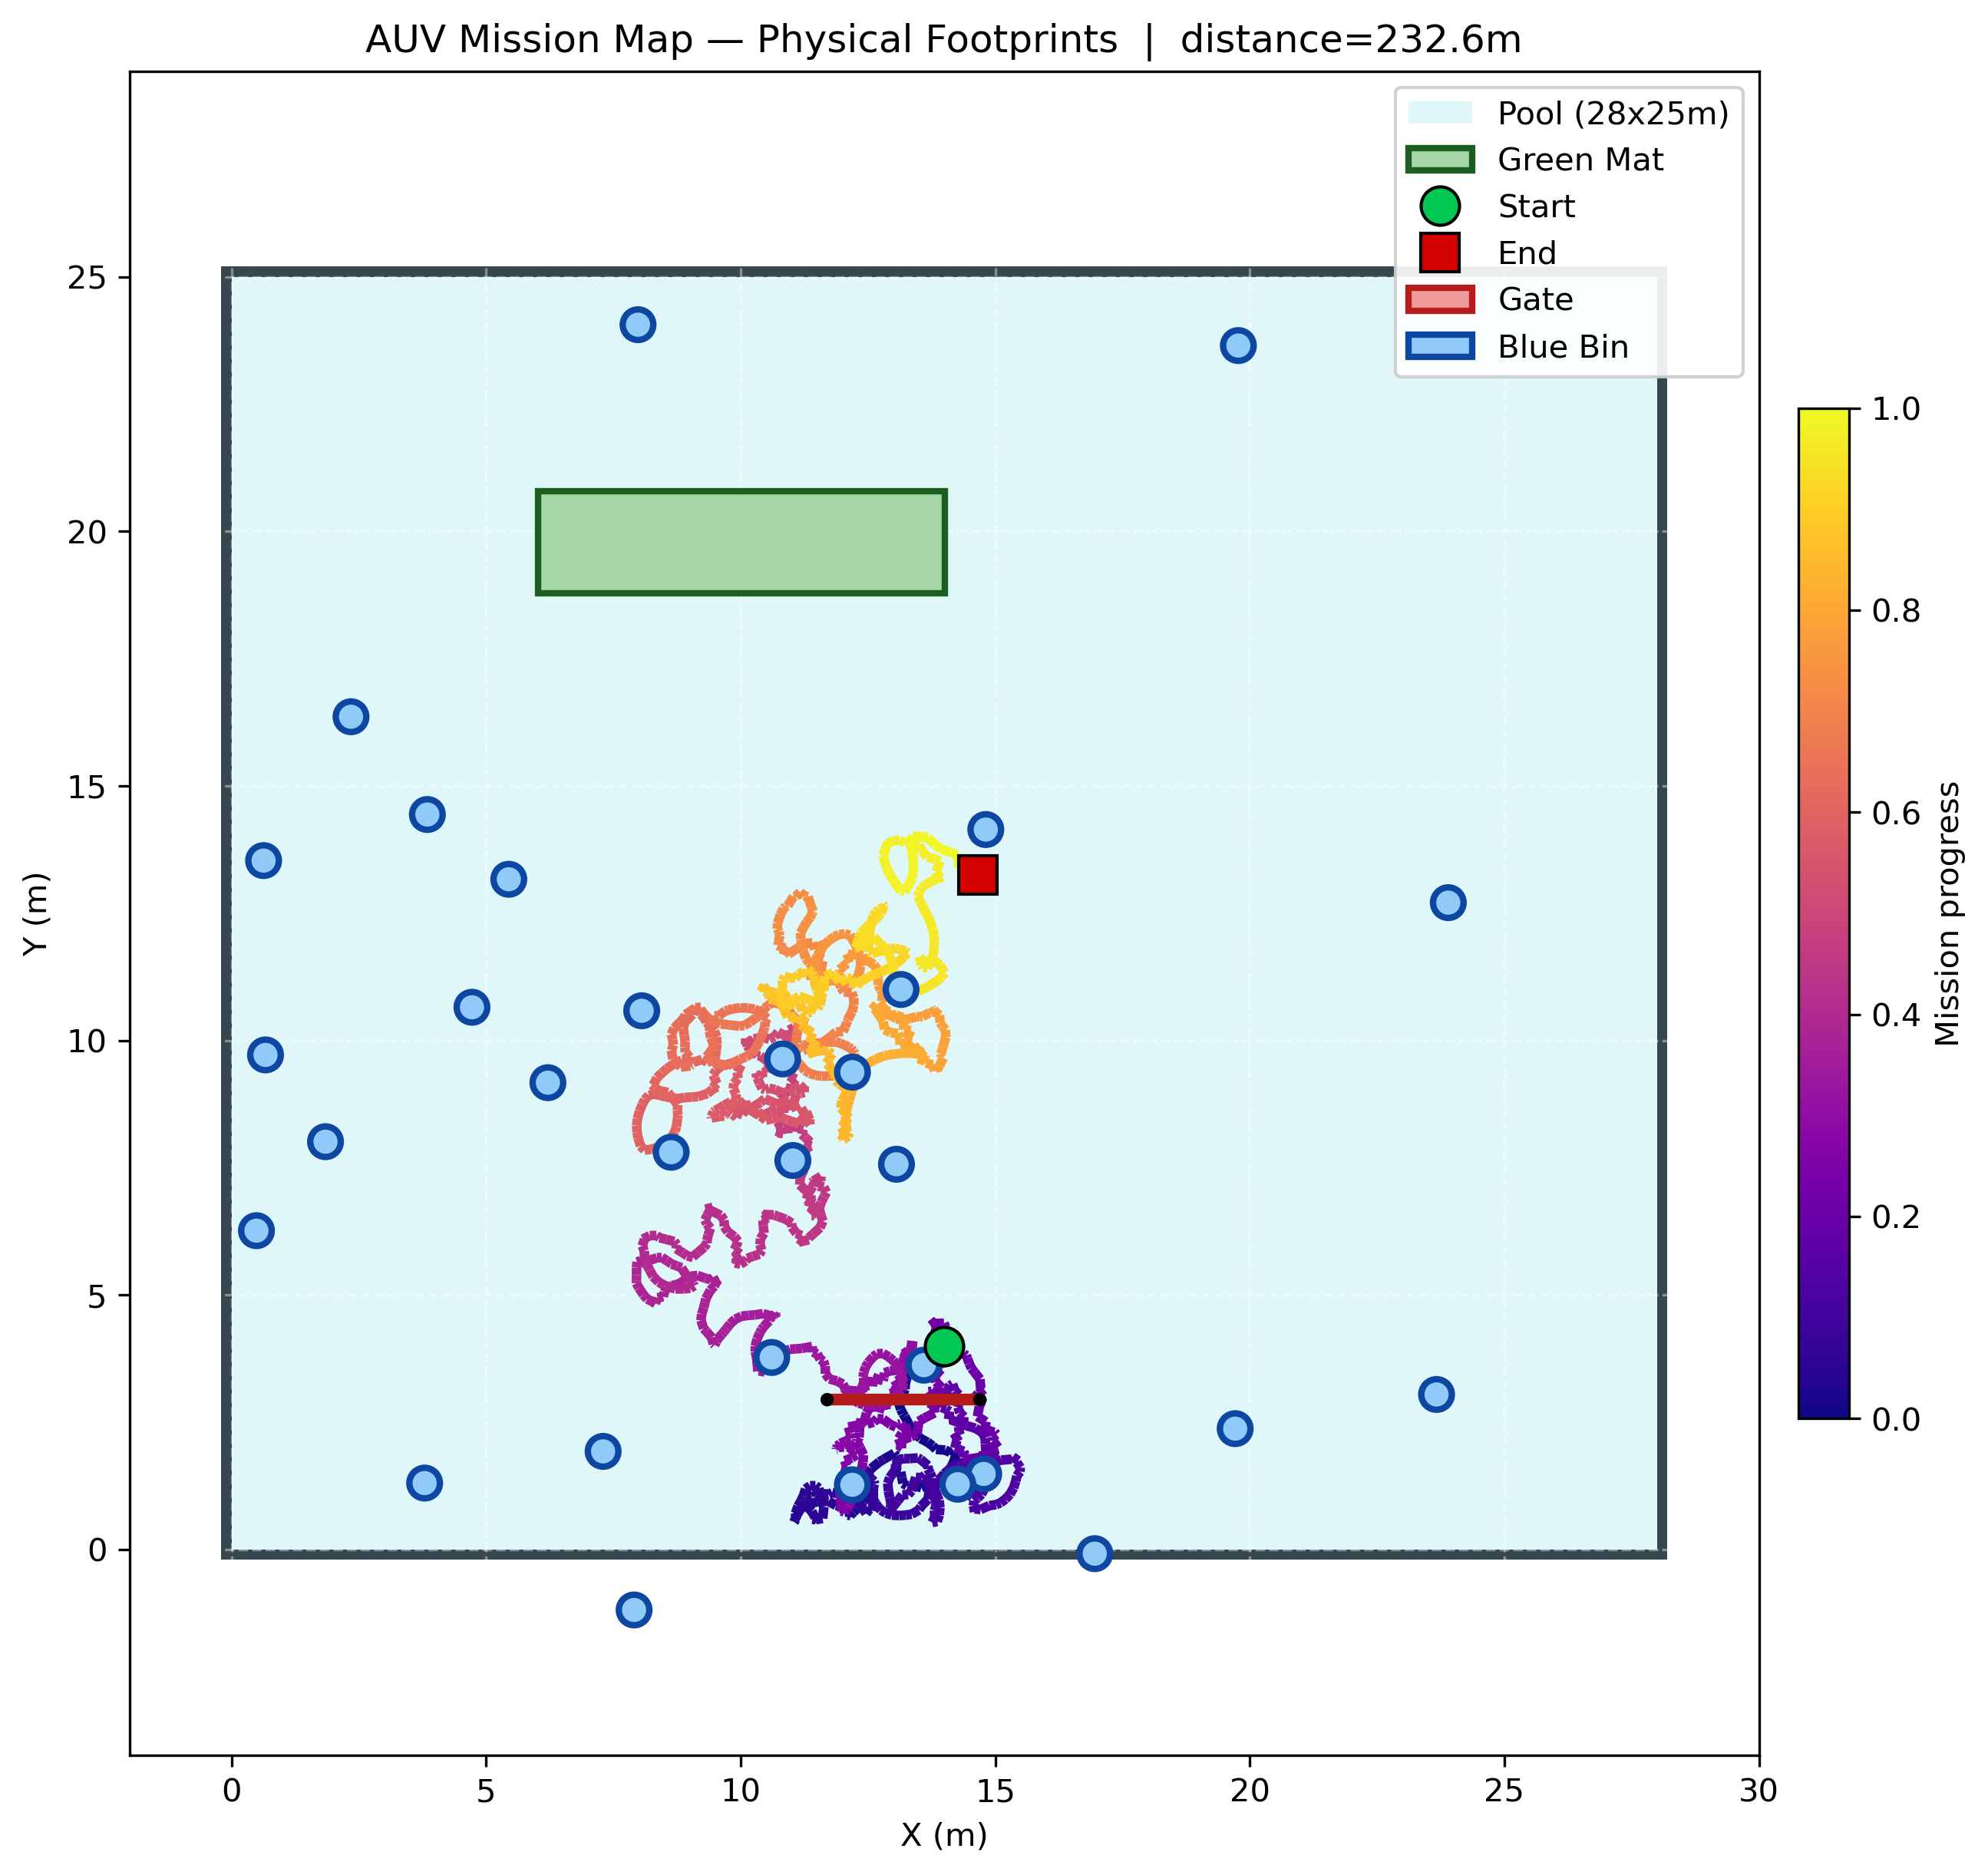
\includegraphics[width=0.66\textwidth]{photos_v2/fig8_mission_map.png}
\caption{Fig 8. Most Recent Mission Trajectory Map (\texttt{map\_20260828\_123328.png}), regenerated from the latest logged run. The trail (yellow=late, purple=early) shows a gate crossing followed by an extended green-mat/blue-bin search phase; the scattered blue-bin markers off the mat reflect transient bottom-camera false detections from that specific run, each independently tracked by \texttt{trail\_mapper\_node}'s per-object association logic rather than a single clean bin fix.}
\end{figure}

This replaces the earlier 45.3\,m single-pass map: the current run covers 232.6\,m because
the post-gate search exercised the full advance-and-sweep budget before converging on the
green mat, which is exactly the behaviour Section~3.2 describes.

%% ============================================================
\section{Summary: What Changed From the Prior Documentation}

\begin{table}[H]\centering\small
\begin{tabularx}{\textwidth}{L{4.3cm} L{5.3cm} X}
\toprule
\rowcolor{tablehead}\textbf{Area} & \textbf{Previously documented} & \textbf{As built today} \\
\midrule
Propulsion & 8-thruster Moore-Penrose allocation, closed-loop wrench controller & Kinematic \code{VelocityControl} plugin; \hl{auv\_controls}/\hl{auv\_propulsion} empty \\
Safety envelope & Tilt damping, depth envelope, wall repulsion & Not implemented anywhere in the stack \\
State estimation & EKF fusing IMU + depth via \code{robot\_localization} & Ground-truth Gazebo odometry only; no IMU modeled, no EKF running \\
Gate TRACK$\to$ALIGN & Commits at a 1.5\,m staging point & Commits at 5.5\,m, held for 5 ticks \\
Gate CROSS overshoot & 3.25\,m & 2.5\,m \\
Post-gate FSM & 8 linear stages incl. \texttt{CLEAR\_GATE} surge \& coverage-based rise & 11-state FSM with advance-and-sweep search and a fixed-altitude survey rise; no \texttt{CLEAR\_GATE} state \\
Red bin / QR & Dedicated detector + localizer nodes & Classes exist in the trained model; no ROS nodes implemented \\
Blue-bin centering & $\pm$20\,px image-space tolerance & 0.30\,m metric tolerance via bottom-camera servoing \\
\bottomrule
\end{tabularx}
\caption{Table: the material differences between the original architecture description and the code in this workspace today.}
\end{table}

\end{document}
